\chapter{Benchmarks}

In this chapter, we measure the performance of our implementation. We quantify the impact of different input size and algorithm parameters. In the end, we compare our implementation with an original python implementation of the algorithm.

All the data was measured using an NVIDIA RTX 3080 graphics card with Intel i5 6600K processor. We used an M.2 SSD AData SX8200 Pro.

To measure the values presented in this chapter, we used a data set provided by the Department of Physics of Material in Charles University in Prague. It contains roughly 15000 electron backscatter patterns --- each of them is a TIFF picture with resolution $873 \times 873$ with color depth of 16 bits. One image has 1.4 megabytes and the whole dataset has 22.3 gigabytes. Most of the testing was performed using only a small subset of the data, since it is needlessly big for most measurements. The exception is the overall comparison to the python implementation and image loading tests for which we needed to use data bigger than the cache of disk.

To measure the performance of individual parts of algorithm we edited the implementation to measure that the respective part takes to complete and write out the average after all the input images (a subset of the 15000 patterns) are processed. So the durations of individual parts are measured directly during running of the whole algorithm. Moreover, we started the whole application several times and again took the average. 

Besides the patterns, the most important input to the algorithm is the description of subregions --- their amount and size of each of them. The actual location of subregions does not have an impact on performance. Throughout the chapter, $S$ denotes the number of subregions. Also, we measure only square subregions, because it removes unnecessary complexity from the benchmarks. In theory, whole algorithm works also for rectangle--shaped subregions, but since we analyze the direction in which the subregions are shifted, the square should have the same dimensions in each direction. Moreover, in this whole chapter, the size of a subregion is half of length of the rectangle side. So for size of subregion $A$, the actual subregion is $2A$ wide and $2A$ high. The reason for this is that the subregion positions determine its middle and it is easier to specify the size as the distance between the middle and sides of the squares.

\section{Relative performance of individual parts}

\begin{figure}
	\centering
	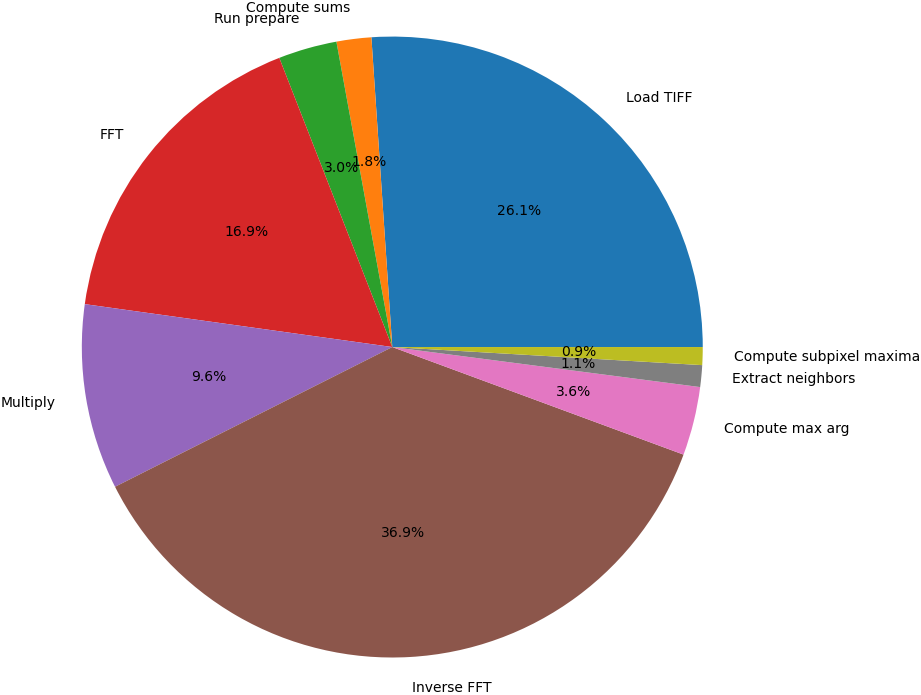
\includegraphics[width=0.7\textwidth]{img/eval/individual-parts}
	\caption{Relative performance of individual parts of the algorithm. The data was measured from a run of the algorithm with a configuration of 90 subregions with size $120 \times 120$. The size of the neigborhood was set to maximal value 9. }
	\label{individual-parts}
\end{figure}

We begin with an overview of all the kernels used in the implementation. \Cref{individual-parts} shows how much time the implementation spends in individual kernels. We can see, that the most demanding parts are loading of the TIFF and the cross--correlation, which is computed using the multiply kernel and the Fourier transforms.

The figure is mentioned here only to get general idea about the performance. It captures relative performance of the kernels for 90 subregions with size $120 \times 120$, which is roughly in the middle of the range of expected values. Different parts depend on different parameters, so for some other input size, the relative performance would look dissimilar. The load TIFF subroutine depends only on the size of the TIFF, while the rest of the algorithm depends on the number of subregion. So, for instance, it is possible to find a configuration that makes load TIFF the longest part. 

\section{Cross--correlation}
First, we measure the performance of cross--correlation when computed using Fourier transform. We show the dependence between running time and size and number of subregions. Since the cross--correlation is computed using three parts, we analyze them one by one. Then we compare the FFT and definition--based implementations.


\subsection{Fourier transforms}
\label{FFT-eval}
\begin{figure}
	\centering
	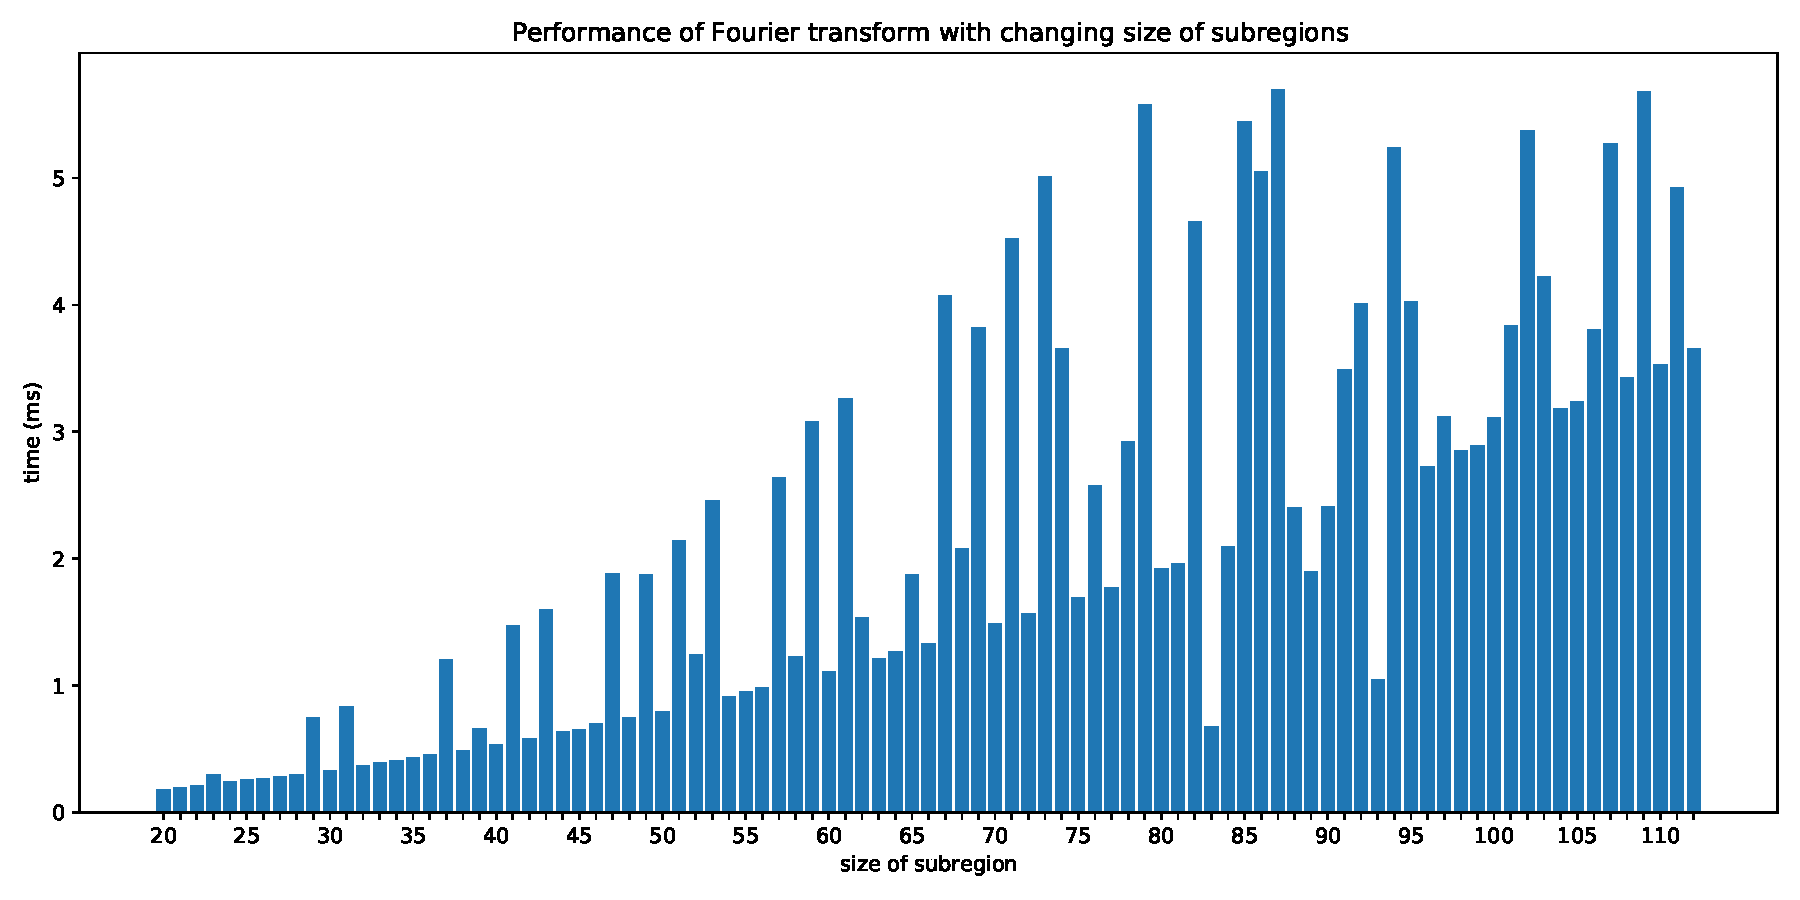
\includegraphics[width=\textwidth]{img/eval/Fourier-transform-size}
	\caption{Performance of Fourier transform with changing size of subregions. It was measured from a run of the algorithm with a configuration of 110 subregions. The size on the x axis denotes half of length of one side of subregion.}
	\label{Fourier-transform-size}
\end{figure}

In the \cref{Fourier-transform-size}, we can see how the forward Fourier transform executed by the cuFFT library depends on the size of subregions. We can see that the computation time increases with the size of the subregions, following the $\mathcal{O}(n \log n)$ time complexity of FFT, where $n$ is number of pixels. More precisely, the complexity is $\mathcal{O}(A^2 \log A)$, if $A$ denotes the length of one side of the square subregion.

However, there are quite a few outliers --- sizes, for which the function does not perform very well. That can be explained by the following sentence cited from the cuFFT documentation: ``Algorithms highly optimized for input sizes that can be written in the form $2^a3^b5^c7^d$''. It means that all sizes, whose factorization contains a prime greater than 7 perform poorly. Choosing a bigger size with nice factorization results in better performance.

We can also see, that sizes 83 and 93 perform surprisingly well. We have measured this fact consistently. The reason behind such behavior is probably specific for cuFFT implementation.

The dependence of inverse Fourier transform on size of subregions looks very similar to the \cref{Fourier-transform-size} for the same reasons.

\begin{figure}
	\begin{subfigure}{.5\textwidth}
		\centering
		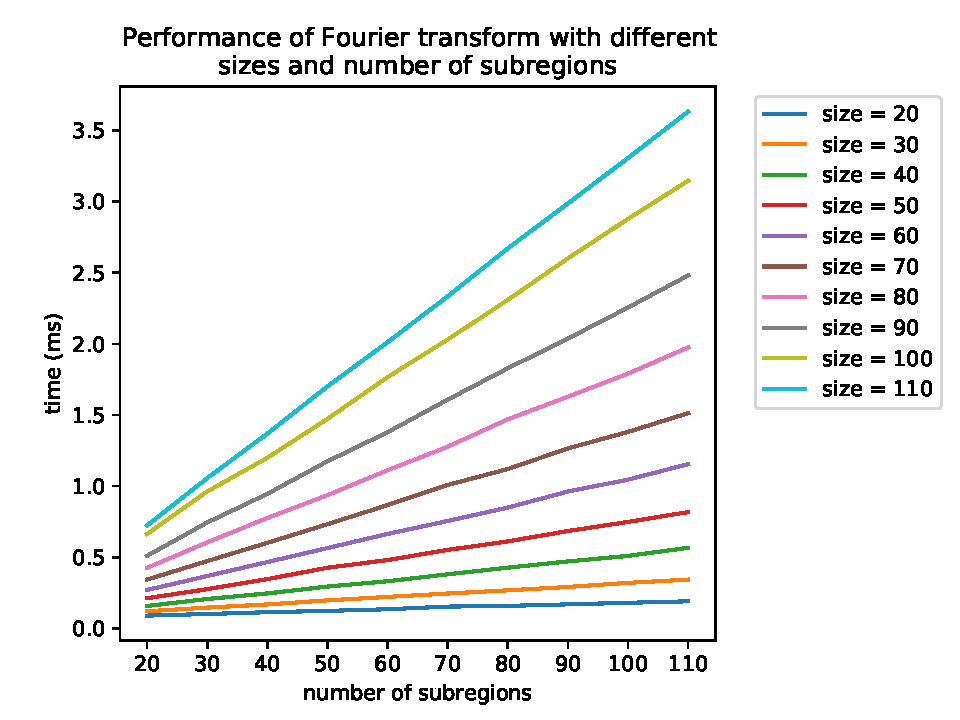
\includegraphics[width=\linewidth]{img/eval/fourier-transform-roi-count}
		\caption{}
		\label{fourier-transform-roi-count:basic}
	\end{subfigure}%
	\begin{subfigure}{.5\textwidth}
		\centering
		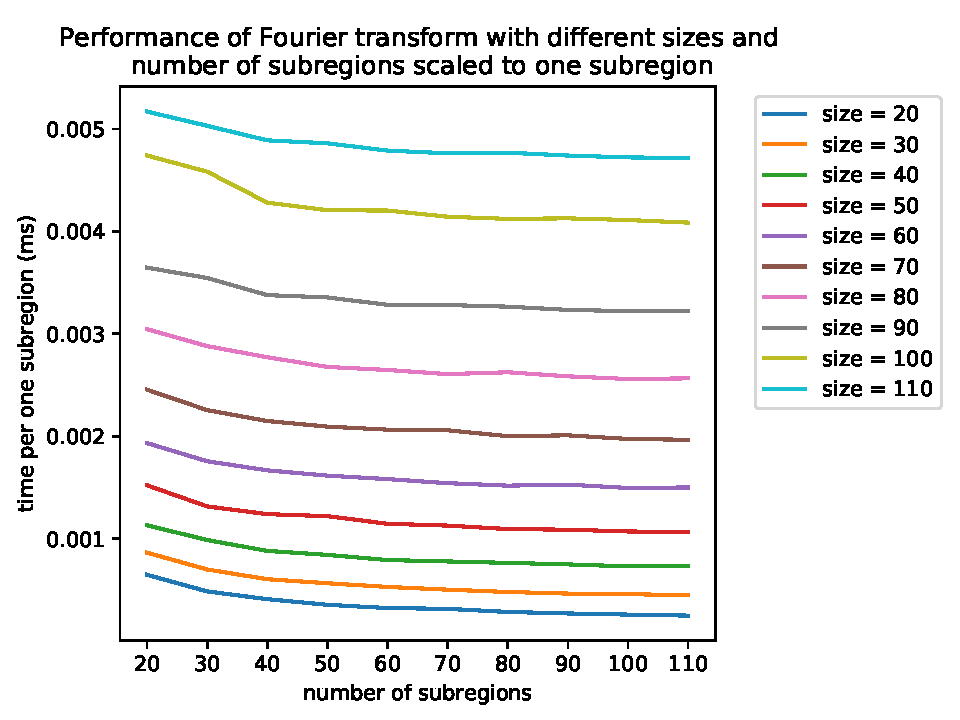
\includegraphics[width=\linewidth]{img/eval/fourier-transform-roi-count-scaled}
		\caption{}
		\label{fourier-transform-roi-count:scaled}
	\end{subfigure}
	\caption{Performance of Fourier transform with changing size and number of subregions. The size on the x axis denotes half of length of one side of subregion.}
	\label{fourier-transform-roi-count}
\end{figure}

\Cref{fourier-transform-roi-count} shows how the the Fourier transform performs with different sizes and number of subregions. \Cref {fourier-transform-roi-count:basic} shows absolute time it takes to compute the Fourier transform. As expected, the time scales roughly linearly with the number of subregions in each image.

\Cref {fourier-transform-roi-count:scaled} shows the same dependence, but the times are scaled with respect to number of subregions, so the y axis shows the average time needed to compute the Fourier transform of one subregion of respectable size. We can see that regardless of the size of subregions the library needs less time per subregion with increasing number of subregions. It is most likely caused by overhead of each CUDA kernel call --- with more subregions, the same overhead is spread over more of them, thus the computation of each subregion is cheaper. That is also the reason why we introduced the batch parameter --- to process more subregions in each run of kernel. We evaluate the impact of the batch parameter to the whole algorithm in \cref{batch-param-eval}.

\subsection{The complex matrix multiplication}
\begin{figure}
	\begin{subfigure}{\textwidth}
		\centering
		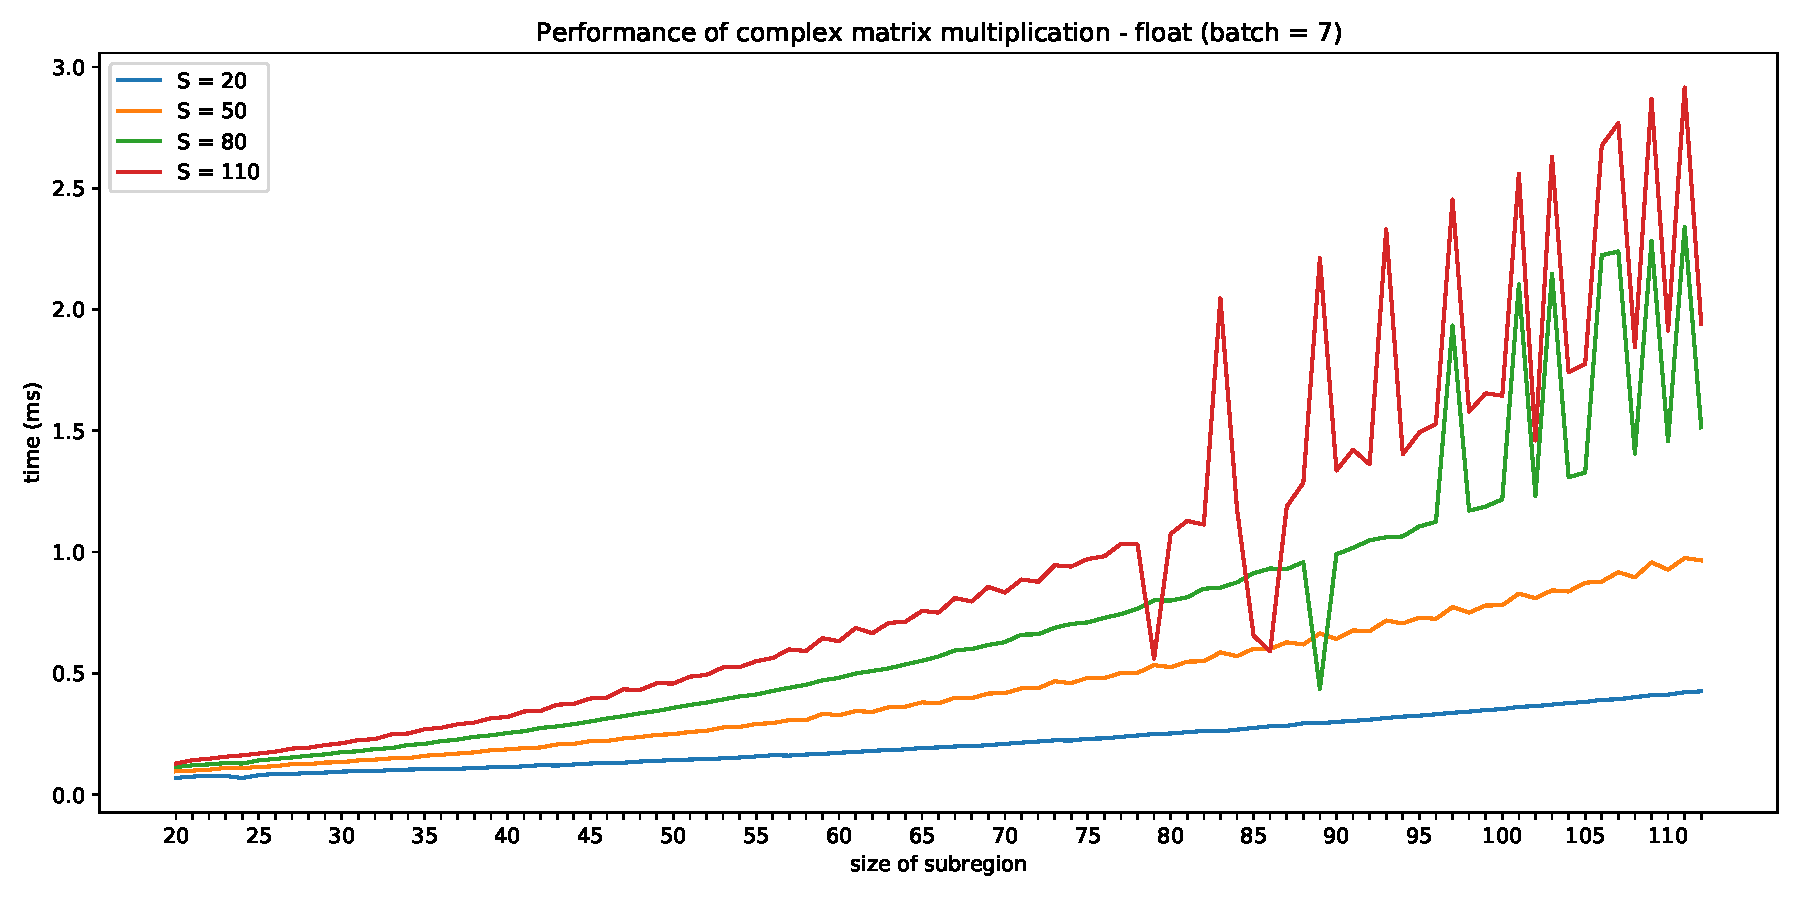
\includegraphics[width=\linewidth]{img/eval/multiply-plot-float}
		\caption{Single float precision}
		\label{multiply-plot:float}
	\end{subfigure}%

	\begin{subfigure}{\textwidth}
		\centering
		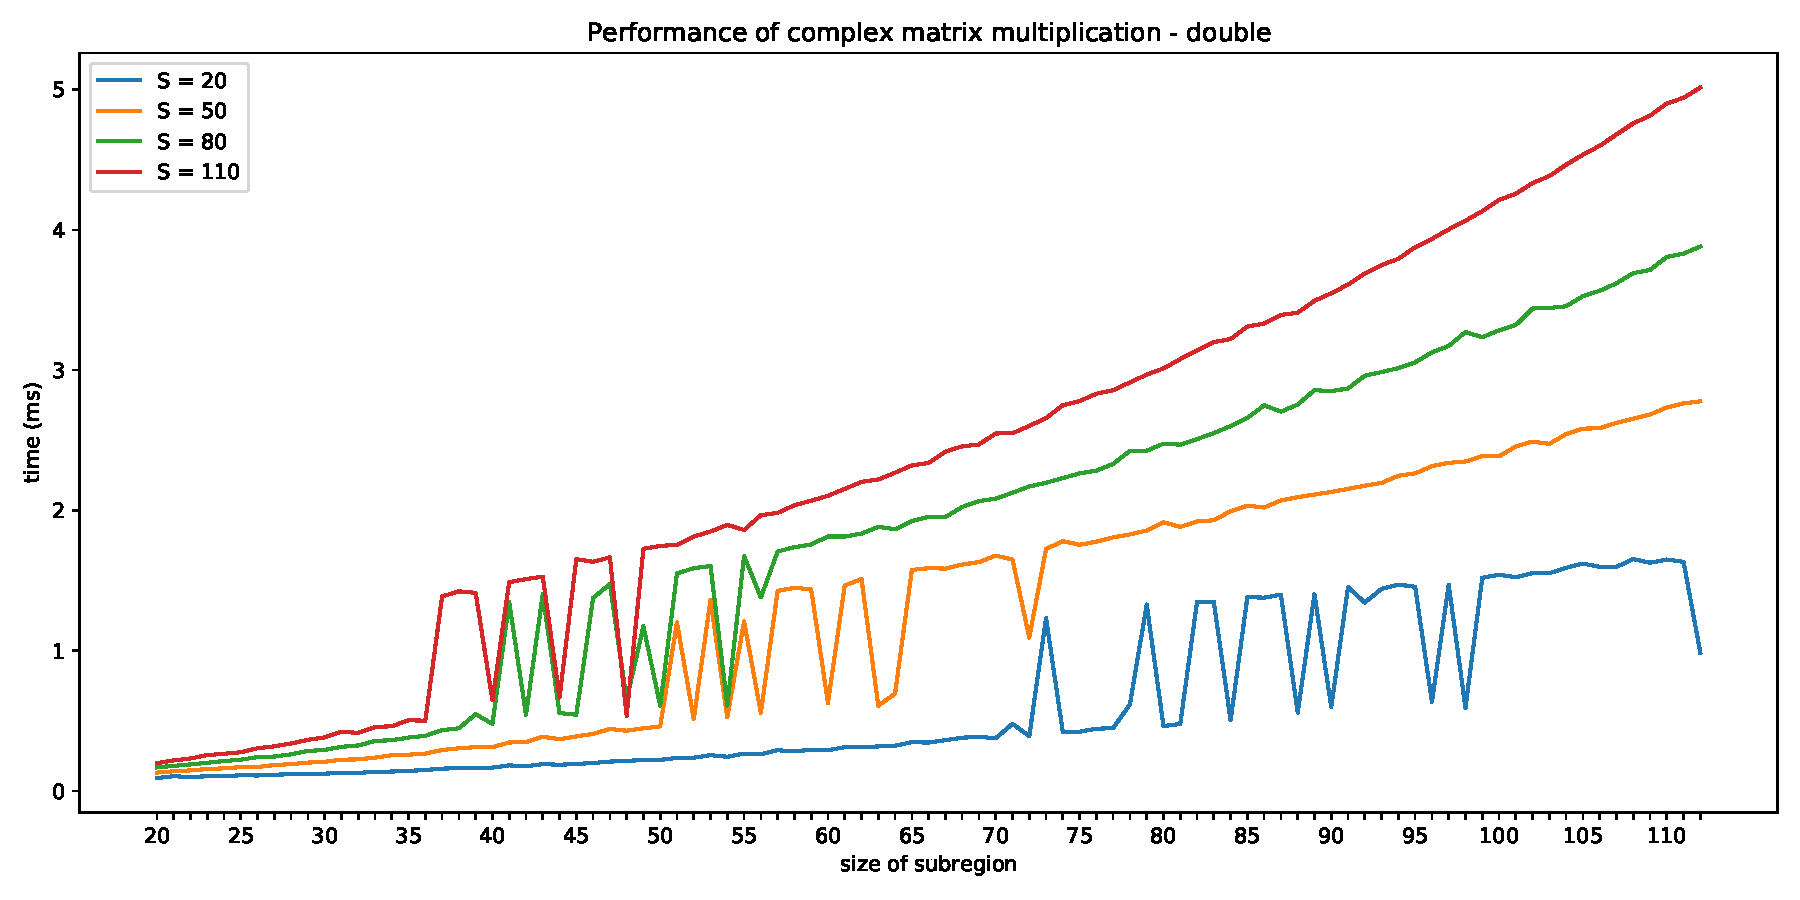
\includegraphics[width=\linewidth]{img/eval/multiply-plot-double}
		\caption{Double float precision}
		\label{multiply-plot:double}
	\end{subfigure}
	\caption{Performance of complex matrix multiplication with changing size and number of subregions. The size on the x axis denotes half of length of one side of subregion.}
	\label{multiply-plot}
\end{figure}

Another step in the cross--correlation computation is the multiplication of two complex matrices. In theory, the complexity of the multiplication is $\mathcal{O}(A^2S)$, where $A$ denotes the length of one side of the square subregion and $S$ denotes their amount. \Cref{multiply-plot} shows the measured time for different sizes and number of subregions. We can see the quadratic trend with respect to subregion size and linear with respect to their count.

However, in some cases, there seem to be a threshold over which the kernel performs worse. For float precision (\cref {multiply-plot:float}), the thresholds are higher than for double precision (\cref {multiply-plot:double}) and we do not see a consistent increase of the time for the measured sizes, only individual spikes. Unfortunately, we cannot reliably determine the relation between the threshold and algorithm parameters. It seems that the data exceed some kind of cache, but we observe worse performance for such big sizes that the processed subregions are already bigger than tens of megabytes. The plots look similar for different batch sizes too.

Moreover, we tried to measure the performance of the multiplication kernel individually and the observed worse performance was not present --- we measured clean quadratic dependency on size of subregions. That implies it is a result of some interference with the cuFFT forward Fourier transform. That would also explain the spikes, since cuFFT behaves differently for sizes with primes in their factorization. In any case, the performance difference is roughly 1ms, which is up to 10\% of total running time of whole offsets computation.

\subsection{FFT implementation versus definition--based implementation}

\begin{figure}
	\centering
	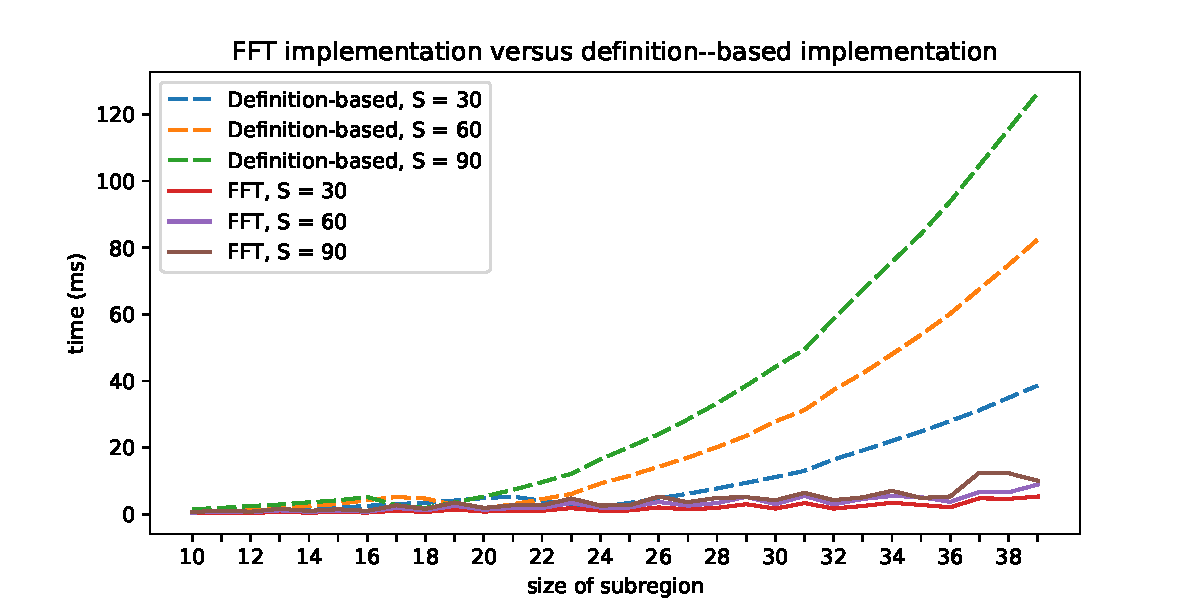
\includegraphics[width=0.8\textwidth]{img/eval/cross-compare}
	\caption{Comparison between the FFT and definition--based implementations of cross--correlation. The size on the x axis denotes half of length of one side of subregion.}
	\label{cross-compare}
\end{figure}

Recall that we described two implementations of cross--correlation: first one based on the Fourier transform and second one based on the definition. \Cref{cross-compare} shows comparison between them --- for the FFT version, it shows the sum of average times of the Fourier transforms and complex multiplication. For the definition--based implementation, it shows the average run time of respective kernel. They are roughly the same for very small subregion sizes, but for sizes bigger than 25 the FFT implementation clearly wins. That is the minimal size of subregions that we consider useful for practical application. The conclusion is that the definition--based implementation is not useful for our application and it is always better to use the FFT implementation. Therefore we use only the FFT implementation in the rest of this chapter.


\section{Pipeline benchmarks}

\begin{figure}
	\centering
	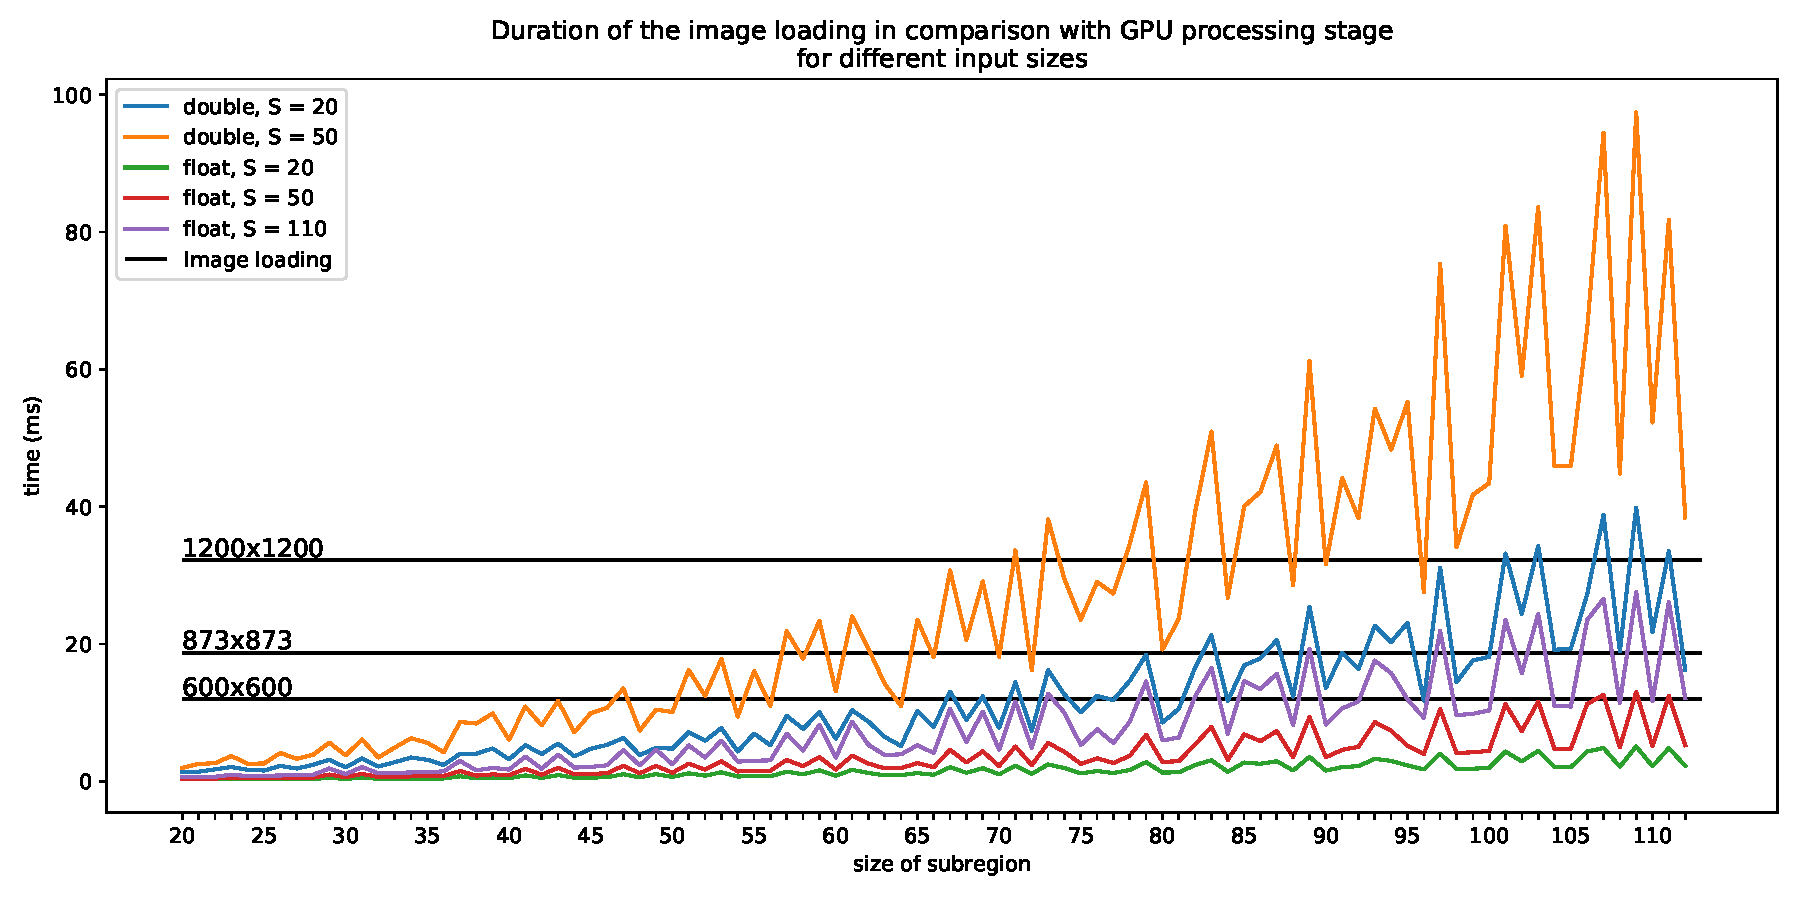
\includegraphics[width=\textwidth]{img/eval/load-plot}
	\caption{}
	\label{load-plot}
\end{figure}

In the following section, we benchmark the pipeline parallelization of pattern loading and GPU processing described in \cref{task-paralelization}. The duration if the image load is simply a linear in number of pixels being loaded, or quadratic function of the width of the image. We show its performance in comparison with the GPU processing time in \cref{load-plot}. There are three black lines which represent the duration of image loading for three different sizes of patterns. They are horizontal, since pattern load does not depend on size of subregions. It was measured using only one CPU thread on a large amount of data, so we ensured that it was not preloaded in disk cache.

Additionally, there are lines that represent the duration of the GPU processing for different number of subregions and floating precision. The GPU processing incorporates all the steps that are implemented for GPU including cross--correlation. For different sizes, we can see the spikes for sizes with primes in their factorization that are explained in \cref{FFT-eval}. Otherwise, the time is increasing with increasing size and number of subregions, as expected.

In the \cref{load-plot}, we can also see which stage of the pipeline is the bottleneck for different parameters. Since the pattern loading and GPU processing are executed simultaneously, whichever of them takes longer is the bottleneck. It is clear that for considerable number of configurations, the amount of data that one thread can load from the disk is insufficient to fully utilize the GPU in the testing computer (it is worth noting that the GPU used is both more expensive and much newer than the CPU). The throughput of the load of images with size $873\times873$ was roughly 500 MB/s, which means we did not fully utilize the used M.2 SSD either.

\subsection{Impact of using more load image threads}

\begin{figure}
	\centering
	\begin{subfigure}{\textwidth}
		\centering
		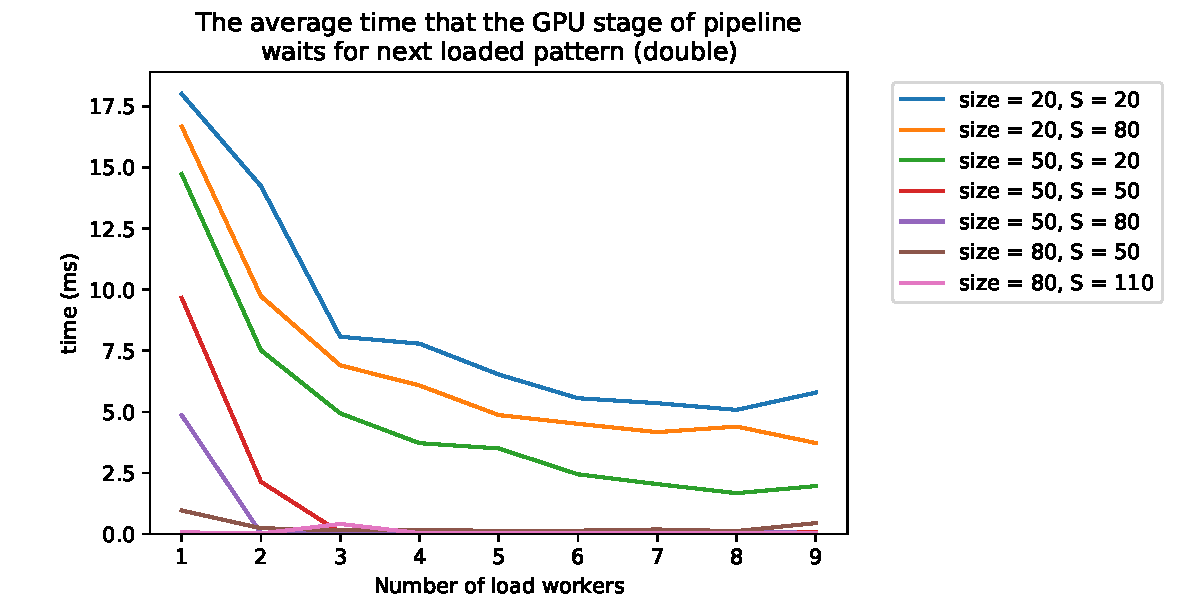
\includegraphics[width=0.75\linewidth]{img/eval/loadworkers-offset-wait}
		\caption{}
		\label{loadworkers-offset-wait}
	\end{subfigure}
	
	\begin{subfigure}{\textwidth}
		\centering
		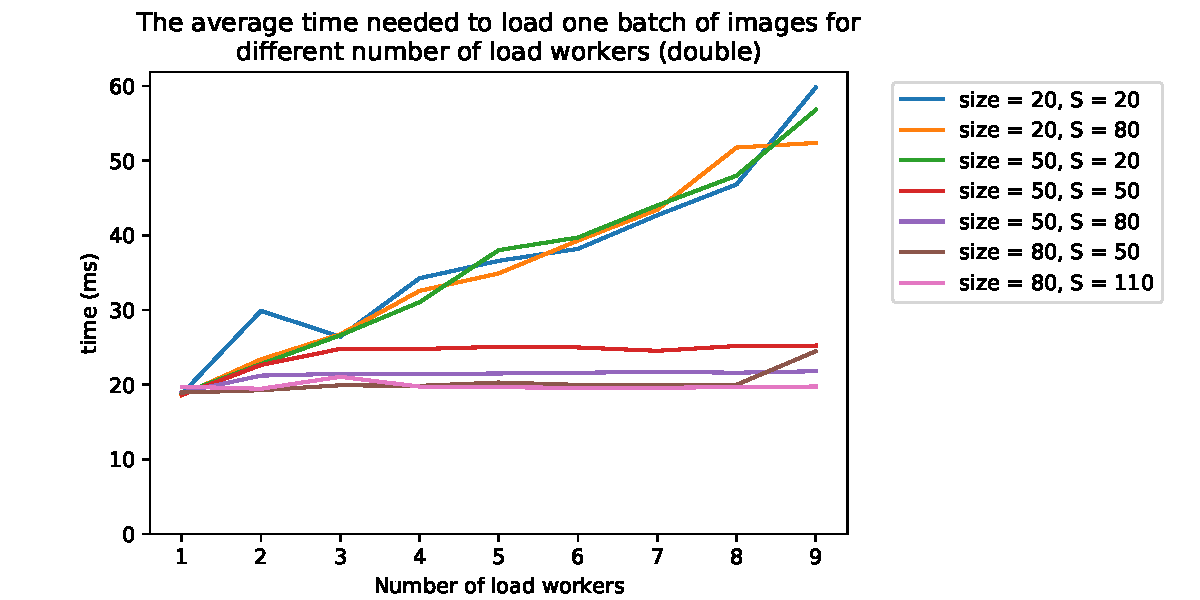
\includegraphics[width=0.75\linewidth]{img/eval/loadworkers-load-tiff}
		\caption{}
		\label{loadworkers-load-tiff}
	\end{subfigure}


	\caption{The average time it takes to load image and the average time the GPU stage waits for loaded patterns, all for different number of load threads.}
	\label{loadworkers}
\end{figure}

\begin{table}[]
	\centering
	\begin{tabular}{@{}l|rrrr@{}}
		S\textbackslash size &      20 &     50 &     80 &   110 \\ \midrule
		20                   & 11710.0 & 2362.8 & 1213.5 & 471.4 \\
		50                   &  6469.3 & 1041.5 &  534.9 & 195.4 \\
		80                   &  4856.7 &  684.6 &  341.7 & 123.3 \\
		110                  &  3765.3 &  515.1 &  251.4 &  90.0
	\end{tabular}
	\caption{Disk throughput needed to fully utilize the tested GPU for different sizes and number of subregions. All the values are in megabytes per second.}
	\label{loadworkers-table}
\end{table}

To utilize the system better, we use several threads to load more patterns simultaneously. The goal is to load the patterns as fast as possible, so that the GPU waits as little as possible. \Cref{loadworkers-offset-wait} shows the average time that the GPU stage waits for the next pattern. We used input images with resolution $873\times873$. We can see that for bigger subregions and bigger number of them, the GPU thread waits less in general. Also, more load workers generally decrease the waiting. And with some of the configurations, more load workers eliminate waiting completely, while the ones with less GPU work cannot fully utilize the GPU even for bigger number of load workers.

To explain the reason why we see two different types of behavior we analyze the throughput of testing system components. \Cref{loadworkers-table} shows the amount of images that the testing GPU is able to process each second in megabytes. To calculate it, we divided the size of one batch of patterns by the measured time it takes to process it by the GPU, which gives us the throughput of loading images that is needed to fully utilize the GPU. To put those numbers in context, a hard disks have read speed of around 100 MB/s, common read speed of SATA SSDs is 500 MB/s and M.2 SSDs can go up to 3500 MB/s. On the testing SSD, we measured read speed of roughly 1500 MB/s when the data was not present in the disk cache.

This information combined with the \cref{loadworkers-table} explains \cref{loadworkers-offset-wait}. For configurations with small number of small subregions (all the configurations with size of 20 and [size = 50, S = 20]), the GPU can process more data than can be loaded from the disk per second. Nevertheless, more load workers allow for better utilization of the disk. For bigger subregions, several load workers are needed to achieve larger disk throughput than the GPU can process and from that point, the GPU does not wait for the image loading anymore.

\Cref{loadworkers-load-tiff} shows the average time that one thread needs to load the image. We can see that for disk--constrained configurations the time each thread needs to load the image increases, as the disk is more loaded. However, at the same time, together they manage to load the images faster. For the GPU--constrained configurations, the load time depends on number of threads needed to utilize the GPU.

All the measured values are, of course, specific to the testing machine. At the same time, it shows that for some configurations, having a fast SSD can be even more important than having a powerful GPU.

\section{Float versus double}


\section{Batch parameter}
\label{batch-param-eval}




\section{Speedup compared to original python implementation}

In the following section, we measure the speedup of the GPU implementation compared to a python implementation provided by Jozef Veselý from Department of Physics of Material in Charles University in Prague. At its core, the implementation relies on FFT implemented in python library scipy. It is able to utilize all CPU cores. Besides that, is uses numpy functions like \texttt{mean} and \texttt{argmax} to perform the additional processing. Thus, the most expensive parts use optimized implementations, but otherwise it is limited by being written in python.

\begin{figure}
	\centering
	\begin{subfigure}{\textwidth}
		\centering
		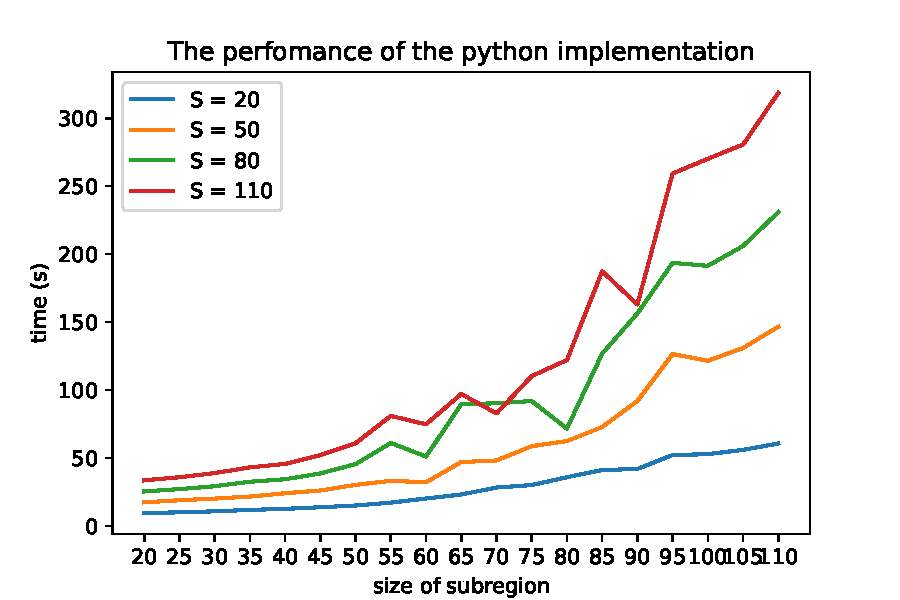
\includegraphics[width=0.75\linewidth]{img/eval/python-impl-plot-abs}
		\caption{}
		\label{python-impl-plot-abs}
	\end{subfigure}
	
	\begin{subfigure}{\textwidth}
		\centering
		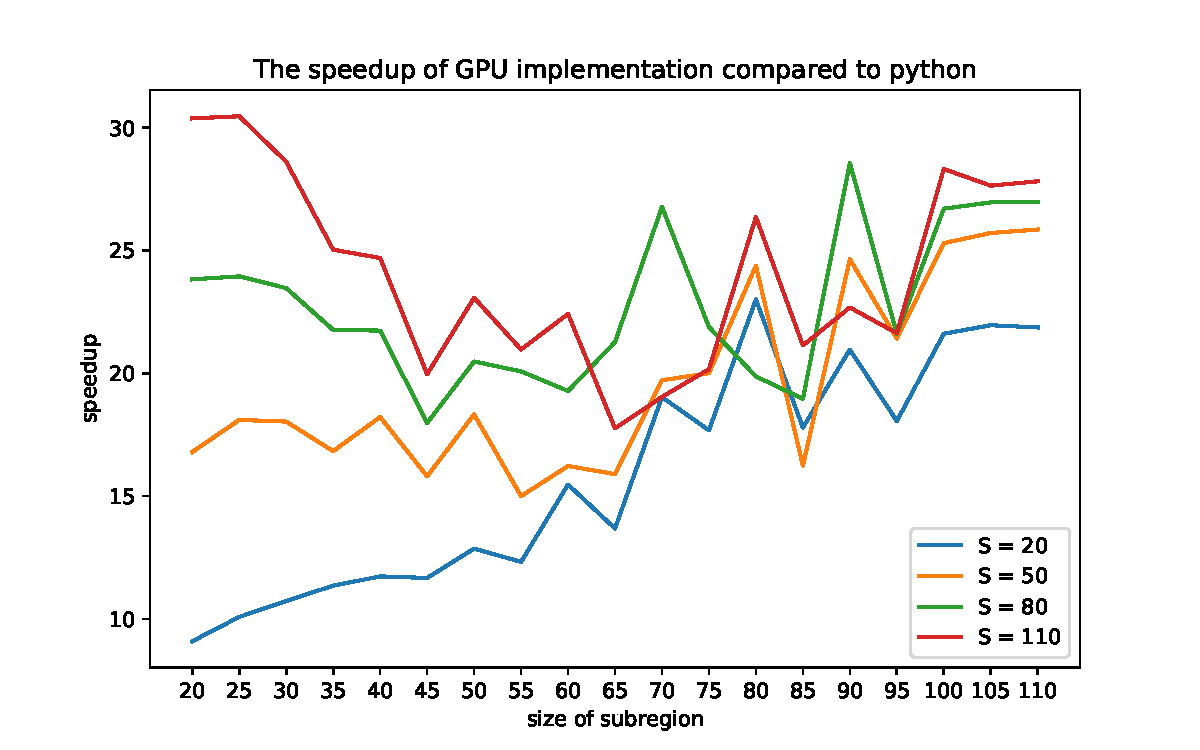
\includegraphics[width=0.75\linewidth]{img/eval/python-impl-plot-speedup}
		\caption{}
		\label{python-impl-plot-speedup}
	\end{subfigure}
	
	
	\caption{The performance of python implementation and its comparison to the GPU implementation}
	\label{python-impl}
\end{figure}

\Cref{python-impl-plot-abs} shows the performance of the python implementation. 

TODO

\section{Memory consumption}


overall performance - compare with python

batch size for different subregion sizes and count

different subregion sizes and count

sum - compare N to size of one slice, to batch size, to number of slices - how?